
\PassOptionsToPackage{svgnames}{xcolor}
\documentclass[11pts,a4paper,amsmath,amssymb,floatfix]{book}
%\usepackage[gather]{chapterbib}

\usepackage{graphicx,wrapfig}% Include figure files
%\usepackage{dcolumn,enumerate}% Align table columns on decimal point
\usepackage{enumerate}% Align table columns on decimal point
\usepackage{bm,dpfloat}% bold math
\usepackage[pdftex,bookmarks,colorlinks=true,urlcolor=rltblue,citecolor=blue]{hyperref}
\usepackage{amsfonts,amsthm,amssymb,stmaryrd,indentfirst}
\usepackage{amsmath}% ,example}
%\numberwithin{Answer}{chapter}
%\numberwithin{Exercise}{chapter
\usepackage{wrapfig}
\usepackage{arydshln}


\usepackage{times,psfrag,pdfpages}
%\usepackage{natbib} 
\usepackage{color}
\usepackage{units}
\usepackage{rotating}
\usepackage{multirow}
% This package provides \cancel{a} and \cancelto{a}{b} to "cancel"
% expressions in math.
\usepackage{cancel}

%\usepackage[sort&compress,square,comma,authoryear]{natbib}
\usepackage[sort&compress,comma,round]{natbib}

% \usepackage{algorithm}
\usepackage[linesnumbered,lined,boxed,commentsnumbered]{algorithm2e}
\usepackage[noend]{algpseudocode} 
\makeatletter
\def\BState{\State\hskip-\ALG@thistlm}
\makeatother

\usepackage{pifont}
\usepackage{subfigure}
\usepackage{subeqnarray}
\usepackage{ifthen}

\usepackage{pgfplots}
\pgfplotsset{every axis/.append style={
                    axis x line=middle,    % put the x axis in the middle
                    axis y line=middle,    % put the y axis in the middle
                    axis line style={<->}, % arrows on the axis
                    xlabel={$x$},          % default put x on x-axis
                    ylabel={$y$},          % default put y on y-axis
                }}



\usepackage{supertabular}
\usepackage{moreverb}
\usepackage{fancyvrb}
\usepackage{listings}
\usepackage{palatino}
%\usepackage{doi}
\usepackage{longtable}
\usepackage{float}
%\usepackage{perpage}
%\MakeSorted{figure}
%\usepackage{pdflscape}
\usepackage{framed,comment,lscape}
\definecolor{shadecolor}{gray}{0.9}

% Appendix allows the inclusion of a line for "appendices", which otherwise won't get the right page number. You must
% use the [toc] option.
%\usepackage[toc]{appendix}

\definecolor{rltblue}{rgb}{0,0,0.75}

%\usepackage{natbib}
\usepackage{fancyhdr} %%%%
\pagestyle{fancy}%%%%
% with this we ensure that the chapter and section
% headings are in lowercase
\renewcommand{\chaptermark}[1]{\markboth{#1}{}}
\renewcommand{\sectionmark}[1]{\markright{\thesection\ #1}}
%\renewcommand*\thesection{\arabic{section}}


\fancyhf{} %delete the current section for header and footer
%\fancyhead[LE,RO]{\bfseries\thepage}
%\fancyfoot[LE,RO]{\bfseries\thepage}
\fancyhead[LO]{\bfseries\rightmark}
\fancyhead[RE]{\bfseries\leftmark}
\renewcommand{\headrulewidth}{0.5pt}
% make space for the rule
\fancypagestyle{plain}{%
\fancyhead{} %get rid of the headers on plain pages
\renewcommand{\headrulewidth}{0pt} % and the line
}

\def\newblock{\hskip .11em plus .33em minus .07em} 
\usepackage{color}

\theoremstyle{definition}
\newtheorem{exmp}{Example}[chapter]

% For theorems
\newtheorem{theorem}{Theorem}[section]
\newtheorem{corollary}{Corollary}[theorem]
\newtheorem{lemma}[theorem]{Lemma}

\usepackage{makeidx}
\makeindex

\setlength\textwidth      {16.cm}
\setlength\textheight     {23.0cm}
\setlength\oddsidemargin  {-0.3cm}
\setlength\evensidemargin {0.3cm}

\setlength\headheight{14.49998pt} 
\setlength\topmargin{0.0cm}
\setlength\headsep{.5cm}
\setlength\footskip{.8cm}
\setlength\parskip{0pt}
%\setlength\parindent{0pt} % no indentation

%%%
%%% Headers and Footers
%\lhead[\text{\small{WORK IN PROGRESS}}] {\text{\small{ICON/AMCG}}} 
%-\lhead[] {\text{\small{ICON/AMCG}}} 
%-\chead[\text{\small{FETCH Manual}}]  {\text{\small{FETCH Manual}}} %{\text{\small{JAERI Analysis Report Issue}}}
%\rhead[]{}
\rfoot[\thepage]{\thepage}
%-\rfoot[]{}%{\text{\small{\today}}}
%\cfoot[\text{\small{\today}}]{}% {\text{\small{\today}}}
%\cfoot[\text{\small{January 2006}}] {\text{\small{January 2006}}}
%-\lfoot []{}%{\text{\small{Numerical Analysis}}}
%-\renewcommand{\headrulewidth}{0.8pt}

%%%
%%% space between lines
%%%
\renewcommand{\baselinestretch}{1.5}

\newenvironment{VarDescription}[1]%
  {\begin{list}{}{\renewcommand{\makelabel}[1]{\textbf{##1:}\hfil}% 
    \settowidth{\labelwidth}{\textbf{#1:}}%
    \setlength{\leftmargin}{\labelwidth}\addtolength{\leftmargin}{\labelsep}}}%
  {\end{list}}

%%%%%%%%%%%%%%%%%%%%%%%%%%%%%%%%%%%%%%%%%%%
%%%%%%                              %%%%%%%
%%%%%%      NOTATION SECTION        %%%%%%%
%%%%%%                              %%%%%%%
%%%%%%%%%%%%%%%%%%%%%%%%%%%%%%%%%%%%%%%%%%%


% This is for quantities which are physically vectors.
\renewcommand{\vec}[1]{{\mbox{\boldmath$#1$}}}
% Physical rank 2 tensors
\newcommand{\tensor}[1]{\overline{\overline{#1}}}
% This is for vectors formed of the value of a quantity at each node.
\newcommand{\dvec}[1]{\underline{#1}}
% This is for matrices in the discrete system.
\newcommand{\mat}[1]{\mathrm{#1}}


\DeclareMathOperator{\sgn}{sgn}

%\newcommand\qed{\hfill\mbox{$\Box$}}
% Derivatives
\renewcommand{\d}{\mathrm{d}}
\newcommand{\D}{\mathrm{D}}
\newcommand{\ddx}[2][x]{\frac{\d#2}{\d#1}}
\newcommand{\ddxx}[2][x]{\frac{\d^2#2}{\d#1^2}}
\newcommand{\ddt}[2][t]{\frac{\d#2}{\d#1}}
\newcommand{\ddtt}[2][t]{\frac{\d^2#2}{\d#1^2}}
\newcommand{\ppx}[2][x]{\frac{\partial#2}{\partial#1}}
\newcommand{\ppxx}[2][x]{\frac{\partial^2#2}{\partial#1^2}}
\newcommand{\ppt}[2][t]{\frac{\partial#2}{\partial#1}}
\newcommand{\pptt}[2][t]{\frac{\partial^2#2}{\partial#1^2}}
\newcommand{\DDx}[2][x]{\frac{\D#2}{\D#1}}
\newcommand{\DDxx}[2][x]{\frac{\D^2#2}{\D#1^2}}
\newcommand{\DDt}[2][t]{\frac{\D#2}{\D#1}}
\newcommand{\DDtt}[2][t]{\frac{\D^2#2}{\D#1^2}}
% Norms

% Units
\newcommand{\m}[1][]{\unit[#1]{m}}
\newcommand{\km}[1][]{\unit[#1]{km}}
\newcommand{\s}[1][]{\unit[#1]{s}}
\newcommand{\invs}[1][]{\unit[#1]{s}\ensuremath{^{-1}}}
\newcommand{\ms}[1][]{\unit[#1]{m\ensuremath{\,}s\ensuremath{^{-1}}}}
\newcommand{\mss}[1][]{\unit[#1]{m\ensuremath{\,}s\ensuremath{^{-2}}}}
\newcommand{\K}[1][]{\unit[#1]{K}}
\newcommand{\PSU}[1][]{\unit[#1]{PSU}}
\newcommand{\Pa}[1][]{\unit[#1]{Pa}}
\newcommand{\kg}[1][]{\unit[#1]{kg}}
\newcommand{\rads}[1][]{\unit[#1]{rad\ensuremath{\,}s\ensuremath{^{-1}}}}
\newcommand{\kgmm}[1][]{\unit[#1]{kg\ensuremath{\,}m\ensuremath{^{-2}}}}
\newcommand{\kgmmm}[1][]{\unit[#1]{kg\ensuremath{\,}m\ensuremath{^{-3}}}}
\newcommand{\Nmm}[1][]{\unit[#1]{N\ensuremath{\,}m\ensuremath{^{-2}}}}

% Dimensionless numbers
\newcommand{\dimensionless}[1]{\mathrm{#1}}
\renewcommand{\Re}{\dimensionless{Re}}

% Other symbols
\newcommand{\frc}{\displaystyle\frac}
\newcommand{\red}{\textcolor{red}}
\newcommand{\blue}{\textcolor{blue}}
\newcommand{\green}{\textcolor{green}}
\newcommand{\purple}{\textcolor{purple}}
\newcommand{\eg}{{\it e.g., }}
\newcommand{\ie}{{\it i.e., }}
\newcommand{\wrt}{{\it wrt }}
\newcommand{\Partial}[3][error]{\left(\frc{\partial #1}{\partial #2}\right)_{#3}}
\newcommand{\mfr}[3][error]{#1_{#2}^{\left(#3\right)}} 
\newcommand{\summation}[3][error]{\sum\limits_{#2}^{#3}#1}

%%%%%%%%%%%%%%%%%%%%%%%%%%%%%%%%%%%%%%%%%%%
%%%%%%                              %%%%%%%
%%%%%% END OF THE NOTATION SECTION  %%%%%%%
%%%%%%                              %%%%%%%
%%%%%%%%%%%%%%%%%%%%%%%%%%%%%%%%%%%%%%%%%%%

% Cause numbering of subsubsections. 
%\setcounter{secnumdepth}{8}
%\setcounter{tocdepth}{8}

\setcounter{secnumdepth}{3}%
\setcounter{tocdepth}{3}%

\usepackage{chngcntr}
%\counterwithout{figure}{chapter}

\newcounter{qcounter}
\newcounter{mcounter}
\DeclareMathAlphabet{\mathpzc}{OT1}{pzc}{m}{it} 

%%%%%%%%%% Chemical Reactions %%%%%%%%%%%%%%%% 

\usepackage[T1]{fontenc}
\usepackage[utf8]{inputenc}
\usepackage{lmodern}
\usepackage[version=3]{mhchem}
\makeatletter
\newcounter{reaction}
%%% >> for article <<
%\renewcommand\thereaction{R6.\,\arabic{reaction}}
%%% << for article <<
%%% >> for report and book >>
\renewcommand\thereaction{R\,\thechapter.\arabic{reaction}}
%\@addtoreset{reaction}{chapter}
%%% << for report and book <<
\newcommand\reactiontag{\refstepcounter{reaction}\tag{\thereaction}}
\newcommand\reaction@[2][]{\begin{equation}\ce{#2}%
\ifx\@empty#1\@empty\else\label{#1}\fi%
\reactiontag\end{equation}}
\newcommand\reaction@nonumber[1]{\begin{equation*}\ce{#1}%
\end{equation*}}
\newcommand\reaction{\@ifstar{\reaction@nonumber}{\reaction@}}
\makeatother

%%%%%%%%%%%%%%%%%%%%%%%%%%%%%%%%%%%%%%%%%%%%%%%%%%%%%%%%%%%%%

%%%%%%%  ENVIRONMENTAL VARIABLES FOR  EXAMPLES     %%%%%%%%%%
\newcounter{examplecounter}
\newenvironment{example}{\begin{quote}%
    \refstepcounter{examplecounter}%
  \textbf{Example \thechapter.\arabic{examplecounter}}% 
  \quad
}{%
\end{quote}%
}
%%%%%%%  ENVIRONMENTAL VARIABLES FOR Tutorial Problems   %%%%%%%%%%
\newcounter{problemcounter}
\newenvironment{problem}{\begin{quote}%
    \refstepcounter{problemcounter}%
  \textbf{Problem \thechapter.\arabic{problemcounter}}%
  \quad
}{%
\end{quote}%
}
%%%%%%%  ENVIRONMENTAL VARIABLES FOR  BLOCKS   %%%%%%%%%%
\usepackage{tcolorbox}
\definecolor{wildblueyonder}{rgb}{0.64, 0.68, 0.82}
\definecolor{whitesmoke}{rgb}{0.96, 0.96, 0.96}
\definecolor{white}{rgb}{1.0, 1.0, 1.0}
\usepackage{lipsum}
\tcbuselibrary{skins,breakable}
\usetikzlibrary{shadings,shadows}
\newenvironment{LearningObjectivesBlock}[1]{%
    \tcolorbox[beamer,%
    noparskip,breakable,
    colback=LightGreen,colframe=DarkGreen,%
    colbacklower=LimeGreen!75!LightGreen,%
    title=#1]}%
    {\endtcolorbox}

\newenvironment{FinalSummaryBlock}[1]{%
    \tcolorbox[beamer,%
    noparskip,breakable,
    colback=LightCoral,colframe=DarkRed,%
    colbacklower=Tomato!75!LightCoral,%
    title=#1]}%
    {\endtcolorbox}

\newenvironment{MyBlock}[1]{%
    \tcolorbox[beamer,%
    noparskip,breakable,
    colback=LightGray,colframe=DarkGray,%
    colbacklower=DarkGray!75!LightGray,%
    title=#1]}%
    {\endtcolorbox}

\newenvironment{MyExample}[1]{%
    \tcolorbox[beamer,%
    noparskip,breakable,
    colback=LightGray,colframe=DarkGray,%
    colbacklower=DarkGray!75!LightGray,%
    title=#1]}%
    {\endtcolorbox}

\newenvironment{MyTutorial}[1]{%
    \tcolorbox[beamer,%
    noparskip,breakable,
    colback=whitesmoke,colframe=whitesmoke,%
    %colback=LightGray,colframe=DarkGray,%
    %colbacklower=DarkGray!75!LightGray,%
    colbacklower=white,%
    title=#1]}%
    {\endtcolorbox}

%%%% ETOC Package to introduce Local Table of Contents
\usepackage{etoc}
\makeatletter
\def\etocarticlestyle{%
    \etocsettocstyle
    {\section *{\contentsname
%                \@mkboth {\MakeUppercase \contentsname}
%                         {\MakeUppercase \contentsname}
         }
         }
    {}}
    \makeatother
    
\makeatletter
\newcommand{\extraPartText}[1]{\def\@extraPartText{#1}}
\pretocmd{\@endpart}{\vspace{8ex}\begingroup\centering\@extraPartText\par\endgroup\let\@extraPartText\relax}{}{}
\makeatother


\begin{document}
\etocsettocdepth{subsection}
\let\cleardoublepage\clearpage

\vspace{4cm}

\begin{titlepage}
  \vspace{3.5cm}

            
\includegraphics[width=15cm,clip]{./FigBanner/UoAHorizBanner}

  \begin{center}

     \vspace{1.cm}

     {\bf{\Huge Lecture Notes on Heat Transfer}} 
     \vspace{1.5cm}
      
      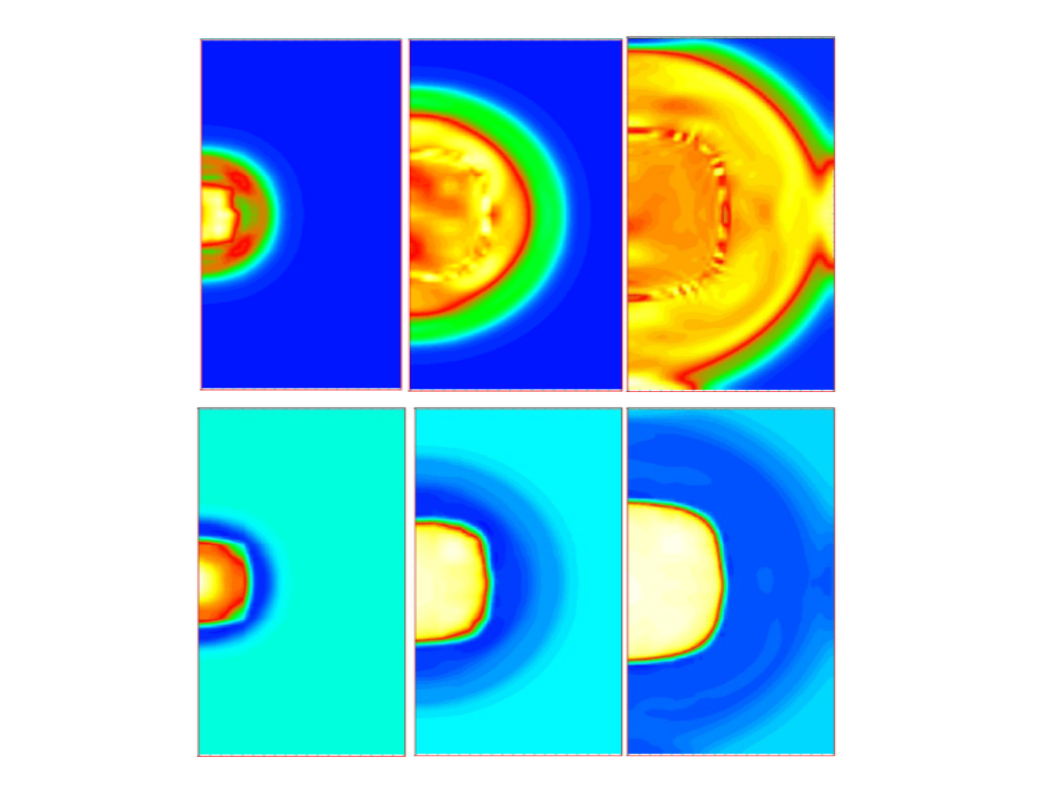
\includegraphics[width=.7\linewidth,height=.5\linewidth,clip]{./Pics/WasteRepos.png}

     \vspace{2cm}
 
     {\Large{\bf \href{tinyurl.com/nlzzbg7}{Jeff Gomes}}}\\
     {\Large{\bf (\href{mailto:jefferson.gomes@abdn.ac.uk}{jefferson.gomes@abdn.ac.uk})}}

     \vspace{1cm}
      {\Large{\bf \href{https://www.abdn.ac.uk/engineering/research/environmental-industrial-fluid-mechanics-122.php}{Mechanics of Fluids, Soils and Structures Research Group}}}
      {\Large{\bf \href{https://www.abdn.ac.uk/engineering/}{School of Engineering}}}\\
      {\Large{\bf \href{https://goo.gl/maps/q3uF9gKyLTN2}{AB24 3UE}}}



     \vspace{2cm}
     {\Large{\bf September, 2017}} %\today}}
  \end{center}

\clearpage

\vbox{
\vspace{18cm}
\begin{description}
  \item[Figure:] Numerical simulation of hypothetical criticality event in nuclear waste repositories. Energetic transients involving extinct fissile material and water surrounded by homogeneous rock matrices (coupled solid-vapour-liquid phase equilibrium and fluid dynamics systems). Extracted from J.L.M.A. Gomes (2009) 'FETCH: A Multi-scale and Multiphysics Model Framework for Nuclear Applications' presented at the 'Todai Forum 2009: Role of Nuclear Energy for Sustainable Development', Imperial College London, UK.
\end{description}}  
\pagenumbering{gobble}% Remove page numbers (and reset to 1)

\end{titlepage} 

%\pagenumbering{roman}% Arabic page numbers (and reset to 1)
\clearpage

\pagenumbering{gobble}% Remove page numbers (and reset to 1)

\pagenumbering{roman}% Arabic page numbers (and reset to 1)
\begin{center}
  \Large{ \bf Revisions}

\bigskip

\begin{tabular}{ c c}
\hline
                         &                    \\
                         &                    \\
{\bf Revision number}    & {\bf Date }        \\
\hline
  0                      & November 5$^{\text{th}}$, 2016   \\
  1                      & August 23$^{\text{rd}}$, 2017    \\
\hline 
\end{tabular}
\end{center}
 
\setcounter{page}{1}

\tableofcontents
\vfill
%%%% ETOC
\etocarticlestyle 

\pagebreak
\listoftables
\vfill
\pagebreak
\listoffigures
\vfill
\pagebreak

\pagenumbering{arabic}% Arabic page numbers (and reset to 1)
\makeatletter\@openrightfalse

     \setcounter{examplecounter}{0}
     \setcounter{problemcounter}{0}
  %%%
%%% CHAPTER
%%%
\chapter{Thermodynamics: Introduction and Principles}\label{Chapter:Introduction}


   \begin{LearningObjectivesBlock}{Learning Objectives}
      Upon completion of this chapter, you will
        \begin{enumerate}
           \item be able to identify the main elements in a thermodynamic system;
           \item understand the concept of thermodynamic equilibrium;
           \item be able to state the zeroth law of thermodynamics.
        \end{enumerate}
\medskip
     Recommended reading: Chapter 2 of \citet{Atkins_Book,Devoe_Book,Borgnakke_Book}.
   \end{LearningObjectivesBlock}

%%%% ETOC
\etocsetnexttocdepth{subsection}
\localtableofcontents

%%%
%%% SECTION
%%%
   \section{Introduction}\label{Chapter:Introduction:Section:Introduction}

 % Transient HT
  %   \setcounter{examplecounter}{0}
  %   \setcounter{problemcounter}{0}
  %\input{Chapter_DesignHE} % Design of Heat Exchangers

\pagebreak 

\cleardoublepage

  \begin{appendix}
     %\part{Appendices} 
       \chapter{Basel Functions}\label{Appendix:BaselFunctions}

Extracted from~\cite{Moran_Book}.

  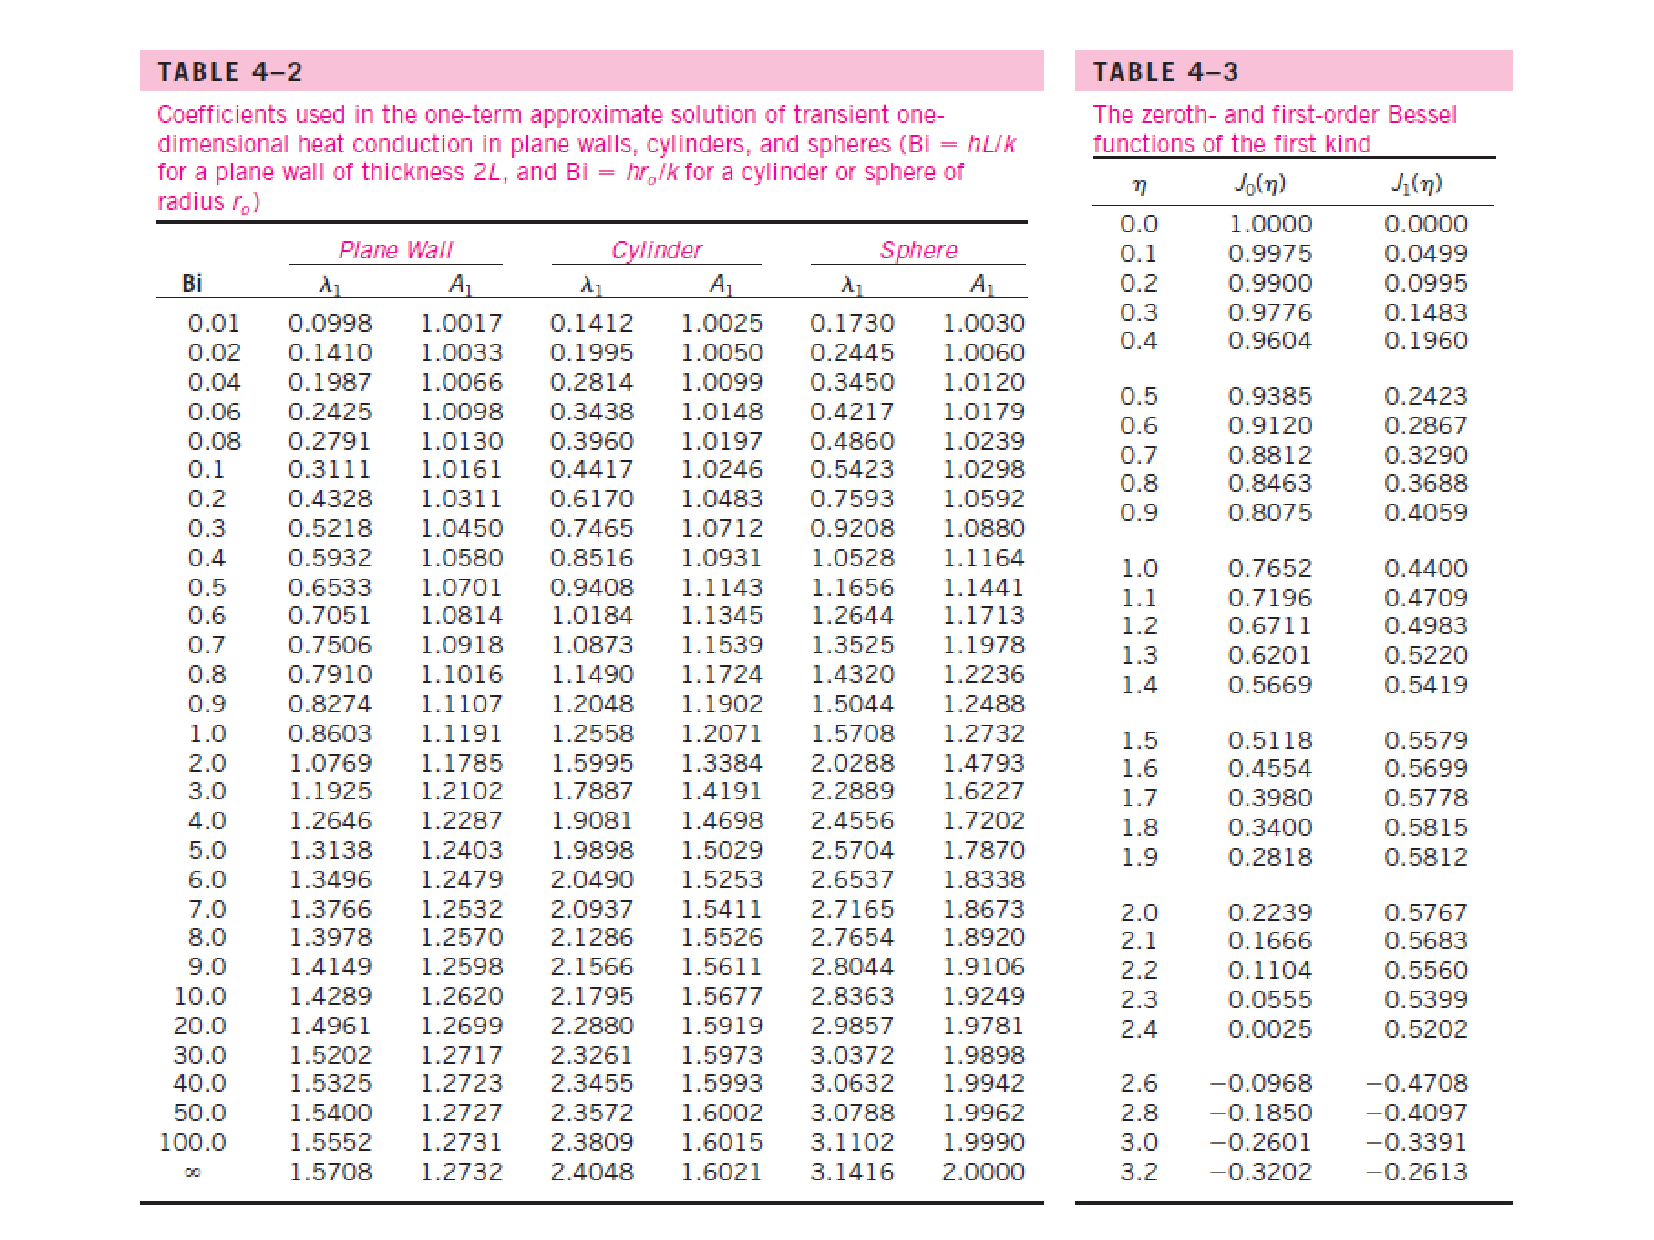
\includepdf[scale=1,pages=-,pagecommand={}, fitpaper]{./Pics/BaselFunctionTable.pdf}

       \chapter{Heisler Charts}\label{Appendix:HeislerCharts}

Extracted from~\cite{Moran_Book}.

  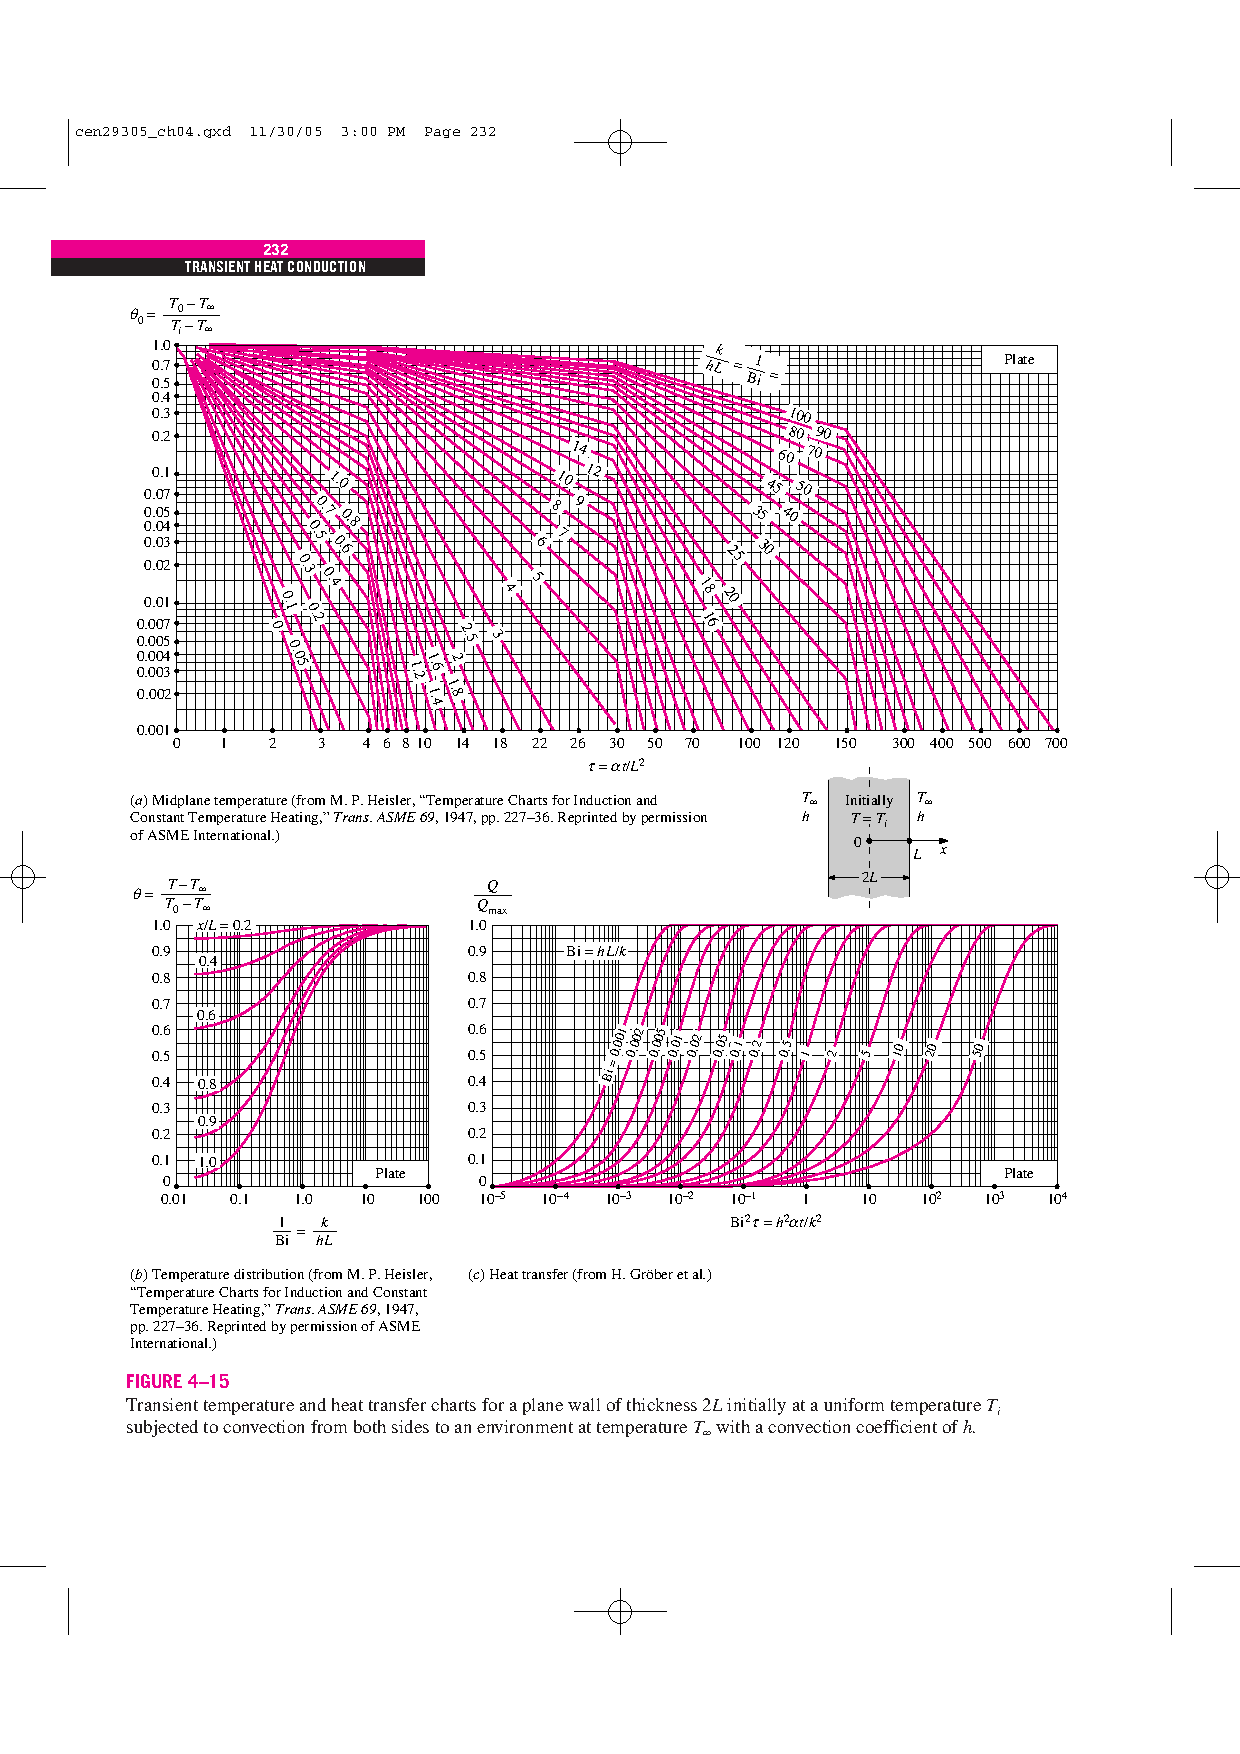
\includepdf[scale=1,pages=-,pagecommand={}, fitpaper]{./Pics/HeislerCharts_All.pdf}

       \chapter{NTU and Efficiency}\label{Appendix:NTU}

Extracted from~\cite{Moran_Book}.

  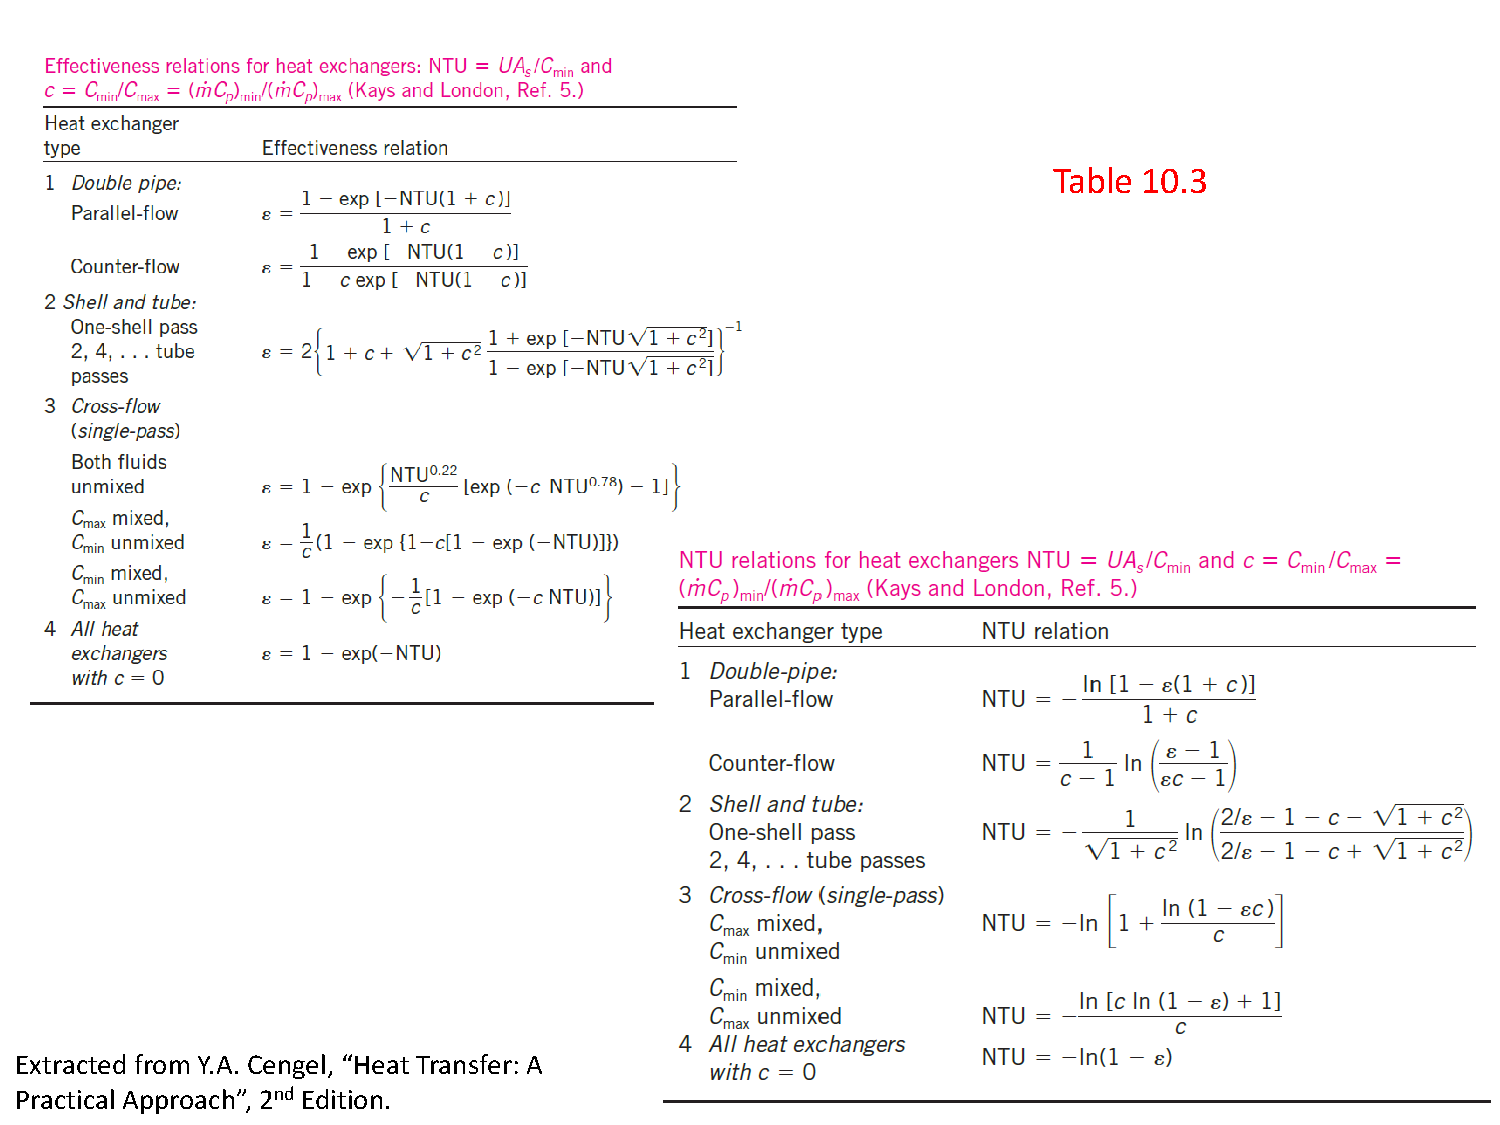
\includepdf[scale=1,pages=-,pagecommand={}, fitpaper]{./Pics/HE_NTU1.pdf}
  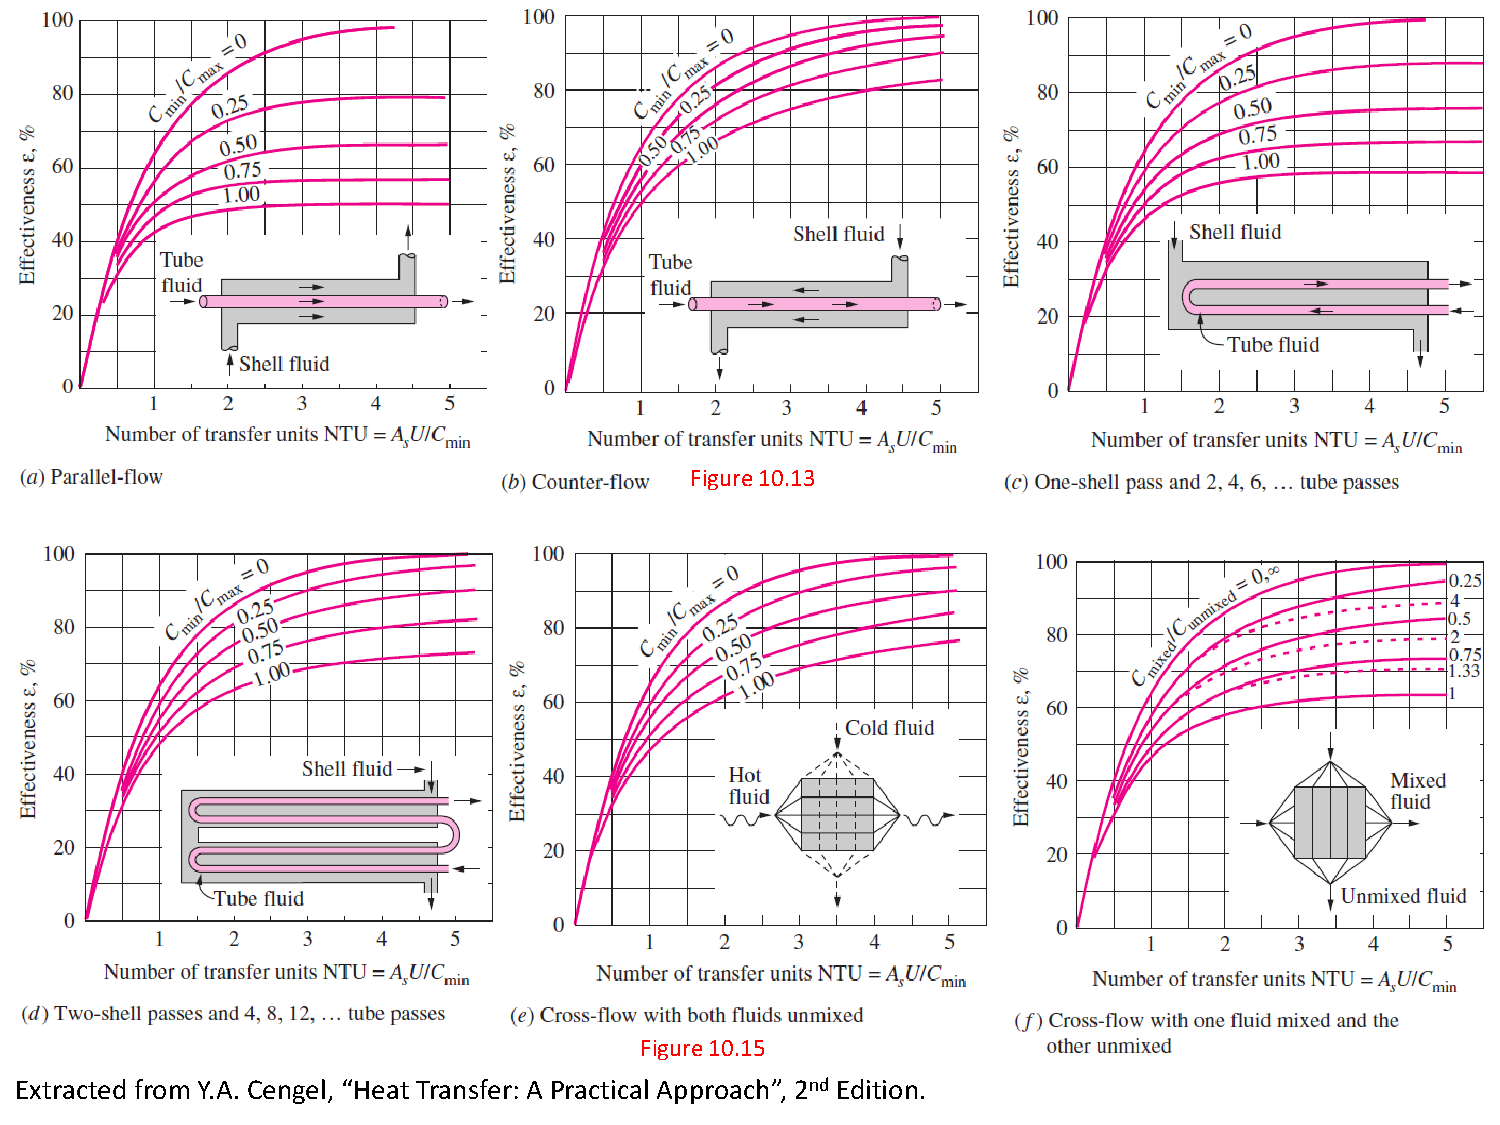
\includepdf[scale=1,pages=-,pagecommand={}, fitpaper]{./Pics/HE_NTU2.pdf}
 
  \end{appendix}

\cleardoublepage

\pagebreak

\bibliographystyle{plainnat}
\bibliography{../refbib}
%\bibliographystyle{unsrt}

\cleardoublepage
\phantomsection
\renewcommand\leftmark{}
\renewcommand\rightmark{Index}
\addcontentsline{toc}{chapter}{Index}

\printindex


\end{document}
